\section{Le conte, vecteur de transmission d'humanisme en déclin}

« Le premier véritable récit est et demeure le conte », Walter Benjamin, Der Erzähler\cite{benjamin1991gesammelte}

\begin{figure}[h!]
    \centering
    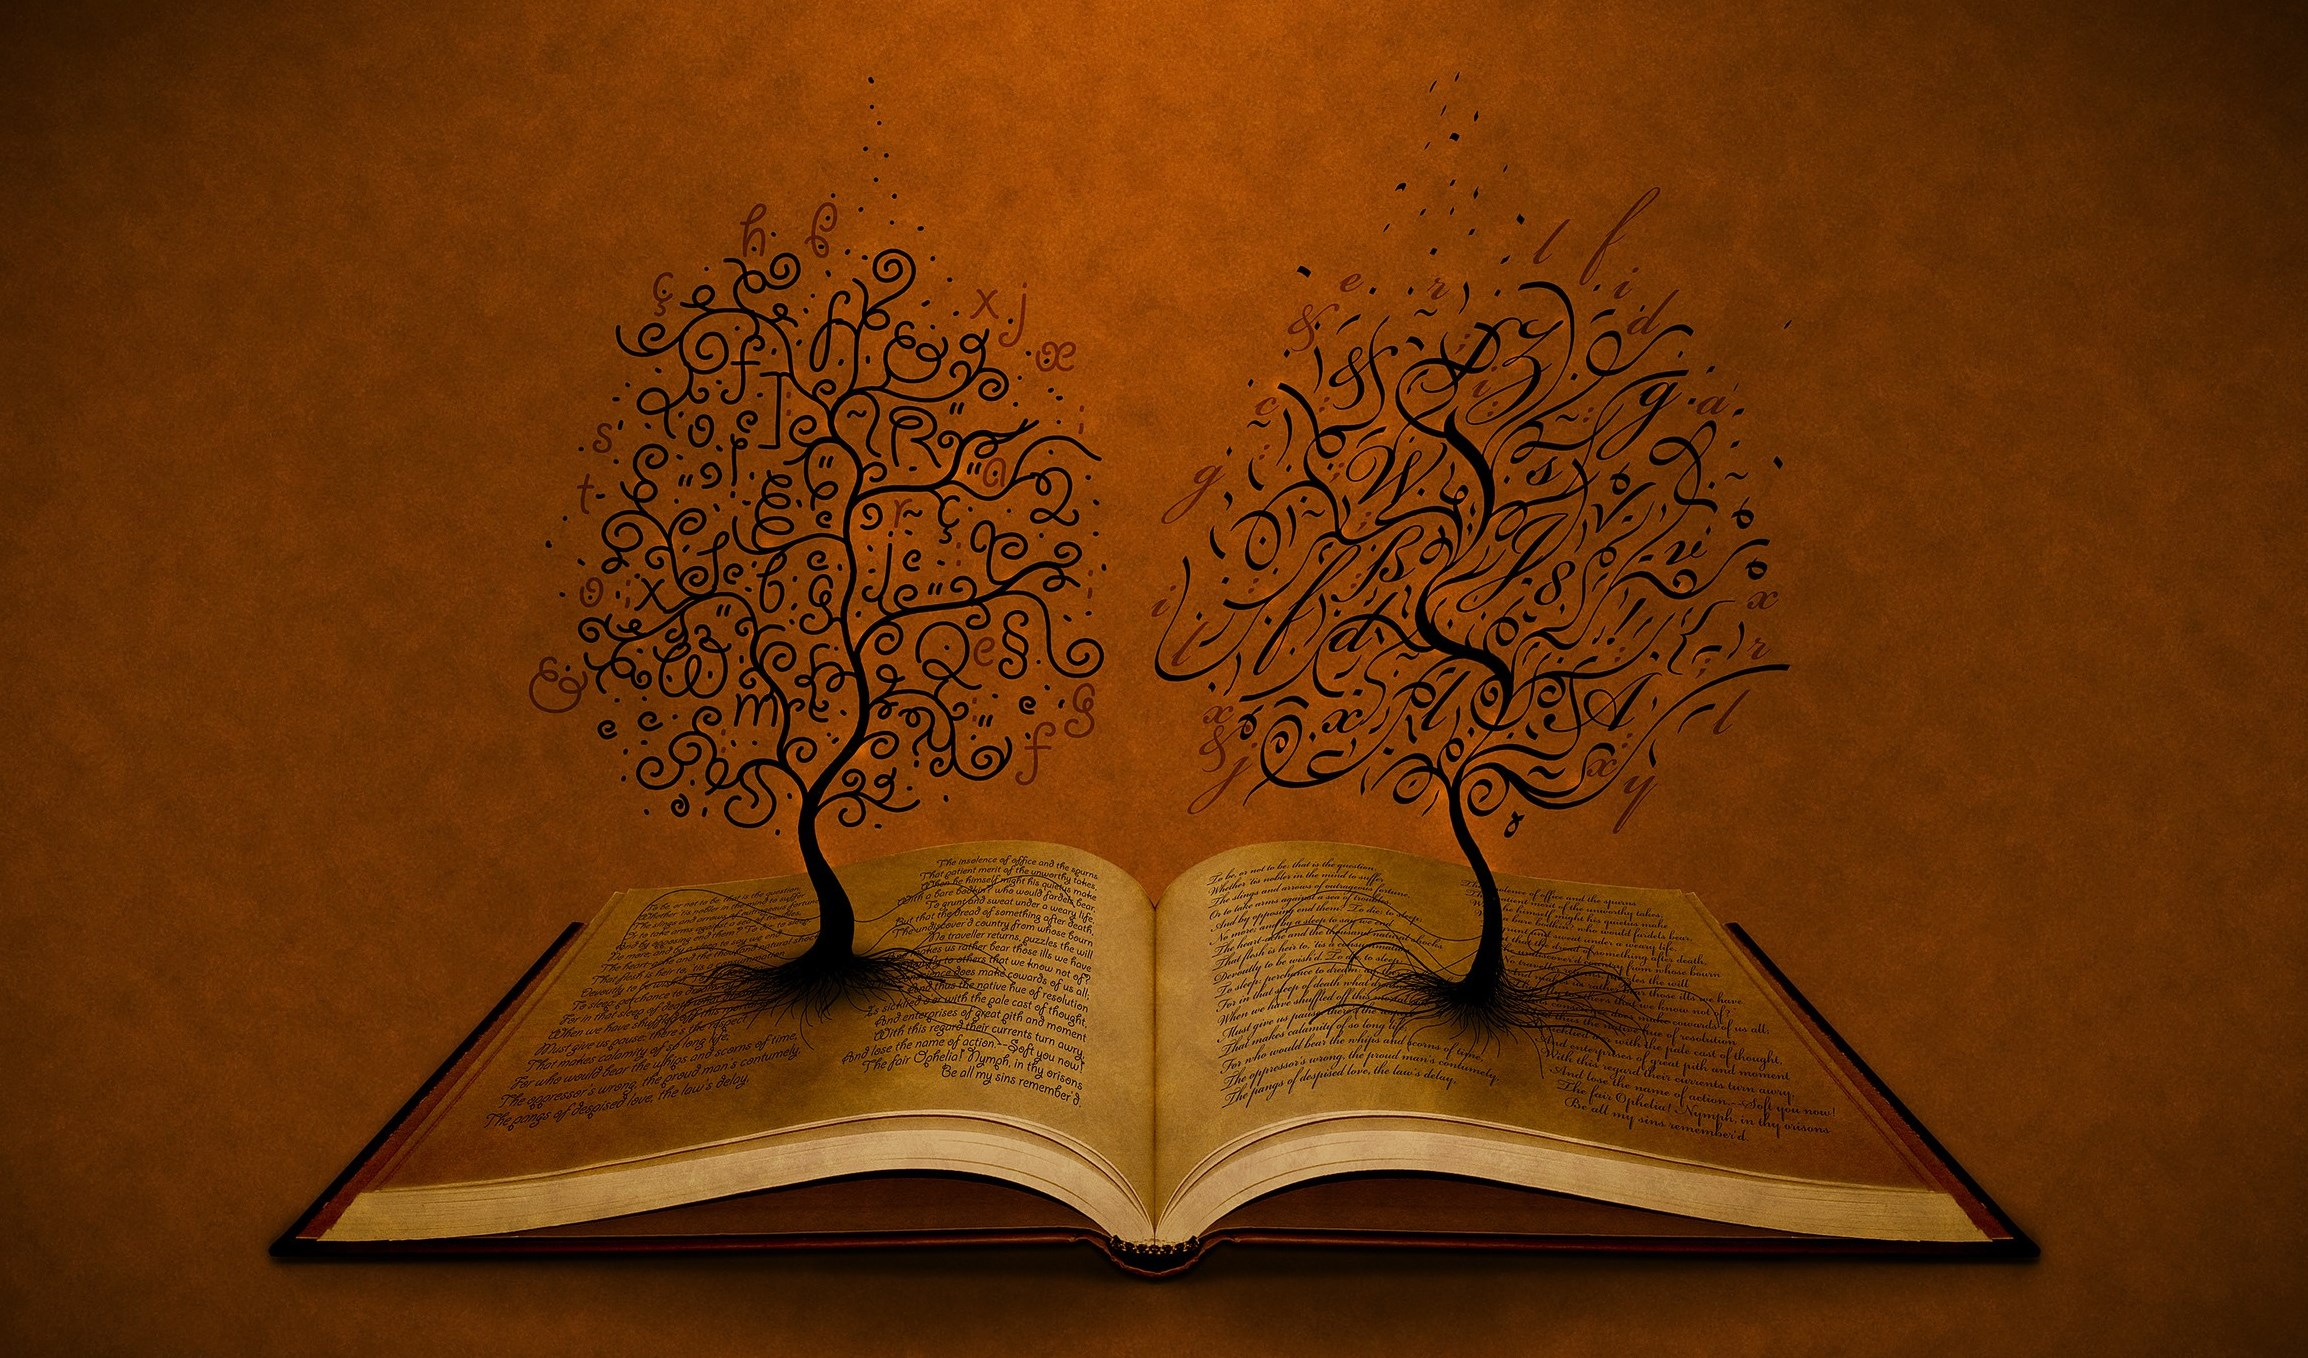
\includegraphics[width=0.80\linewidth]{img/tale_book.jpg}
    \caption{Tale book}
\end{figure}

\subsection{Porteur d'expérience}
Conteur = narrateur\\
Conte opposé au mythe\\
Littérature orale\\

Interprétation Calter Benjamin : \cite{nouss2003conteur}
On parle ici de contes oraux essentiellement
Anciennement et encore aujourd'hui, le conte était un vecteur de perpétuation de l'expérience et de renouvellement de la tradition
La transmission orale via le conte est en perte de vitesse (Walter Benjamin) car elle est essentiellement relative à la transmission d'une expérience, dont l'intérêt porté est en net déclin.\\
Conteurs : sédentaire (perpétuant un lointain temporel constitué de riches expériences passées) / voyageur (rapportant un lointain spatial d'expériences vécues ou entendues en d'autres lieux)\\

L'expérience ici mentionnée peut faire référence à un récit véridique ou bien façonné, porteur d'une morale visant à enrichir l'auditoire du passé, dans le but de guider celui-ci dans les choix futurs qui se poseront à lui.\\
Par ailleurs, le conteur est dans un rapport de proximité avec son auditoire, ce qui permet l'exposé de la distance.\\
Or, cette recherche d'expérience est en perte de vitesse, notamment de par l'information journalistique informant tout un chacun des derniers évènements survenus, prémachés, analysés et expliqués. Au contraire, le conte laisse l'auditoire tirer ses propres conclusions. Le conte délivre en effet un fait nu, exempte de toute explication. La valeur du conte ne réside plus alors dans son intrigue, mais dans la mise en valeur de l'acte de vivre une expérience à proprement parler. C'est donc une conception de l'être humain qui est ainsi véhiculée, celle de vivre des expériences, de traverser des épreuves, et de les surmonter.\\

\begin{figure}[h!]
    \centering
    
\includegraphics[width=0.80\linewidth]{img/storyteller.png}
    \caption{Storyteller}
\end{figure}

\subsection{L'écoute flottante (à détailler ?)}
Dans l'écoute du conte, le procédé freudien d'attention flottante consistant en l'absence d'attention dirigée ou focalisée, permettrait à l'auditeur de s'oublier lui-même, afin que «les mots qu'il entend[e] s'inscrivent profondément en lui» (ibid), facteur essentiel de l'assimilation et de la mémorisation des contes par l'auditoire via une écoute détendue.\\

\subsection{Le conte et la mort (reformuler)}
«Le parfait récit naît de l'accumulation de ses versions successives». Chaque conteur apose en effet sa marque au récit, transformant celui-ci de par son vécu.\\
L'existence d'un conte réside dans la mémoire de son auditoire, sa survie dans la transmission perpétuée par ses conteurs. Un conte meurt s'il n'est pas transmis.\\
Une cause cause annexe de déclin pourrait résider dans la conception de la mort par l'humain.\\
Selon W. B., le conteur tient de la mort son autorité. En effet, les contes étant faits de vécu, une vie d'expériences fondera donc une sagesse ou un savoir dont la transmission sera d'autant plus riche que la vie en fut emplie :  «La mort est la sanction de tout ce que relate le conteur». À l'heure de sa mort, toute personne devient donc digne d'être écoutée.\\

Le siècle dernier aurait néanmoins bouleversé la conception sociale de la mort dans nos moeurs. Les progrès technologiques et les atrocités commises ont eu pour effet l'acceptation de la conception d'une mort en masse (Hiroshima), pleine de souffrances (camps de déportation), banalisée et quotidienne (médias).\\
La mort étant transformée, l'autorité qu'on en retire en tant que conteur en est également impactée.\\
Les évènements passés ayant bouleversé le rapport mort/vie, ceux-ci ont également impacté la conception que tout un chacun se fait de la survie. La mort d'un être humain conte revêt alors une importance bien moindre, de même que celle d'un conte.

\clearpage
